\chapter{Access to the VSC Cloud}
\section{Requirements}\label{sec:requirements}
Before you try to access the VSC cloud services, please ensure the following:
\begin{itemize}
\item You have an active VSC account.  New users can obtain an account
  at \url{https://www.vscentrum.be/cluster-doc/account-request}.
\item Your account is part of one or more OpenStack projects.  Please
  contact \cloudinfo if you want to start a new project or join an
  existing one.
\end{itemize}

\section{Login}\label{sec:access}
Your cloud resources are managed using a web interface, which you can access via \url{https://cloud.vscentrum.be}.

To log in, choose the (default) authentication method \emph{VSC Accountpage} and click \strong{Connect}.
\begin{center}
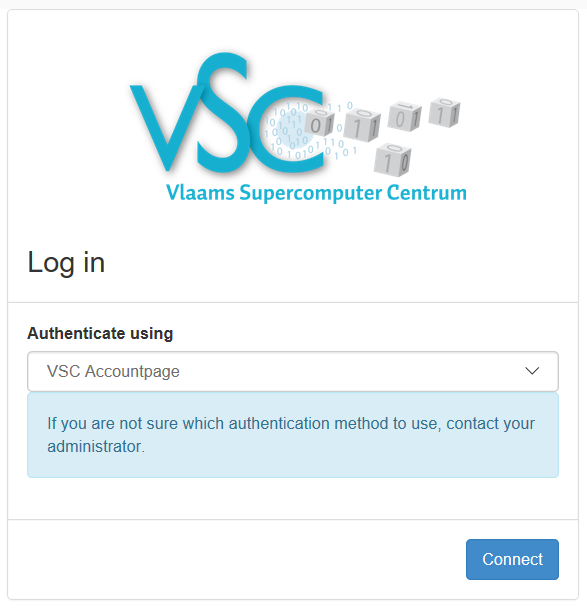
\includegraphics[width=0.5\textwidth]{img/cloud_login_1.png}
\end{center}

From here on, follow the standard procedure to log in to your VSC account, using your home institution's central sign-on system.  You can find a detailed description in the HPC tutorial at \url{https://vscentrum.be/support/tut-book/vsc-tutorials}.

%%% Local Variables:
%%% mode: latex
%%% TeX-master: "intro-OpenStack"
%%% End:
